\begin{figure}[ht]
\centering
\subfigure[]{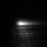
\includegraphics[width=4cm,keepaspectratio]{interference/figures/move/321-1.png}}
\subfigure[]{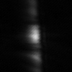
\includegraphics[width=4cm,keepaspectratio]{interference/figures/move/321-2.png}}
\subfigure[]{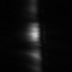
\includegraphics[width=4cm,keepaspectratio]{interference/figures/move/321-3.png}}\\
\subfigure[]{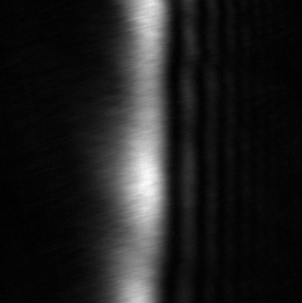
\includegraphics[width=4cm,keepaspectratio]{interference/figures/move/321-7.png}}
\subfigure[]{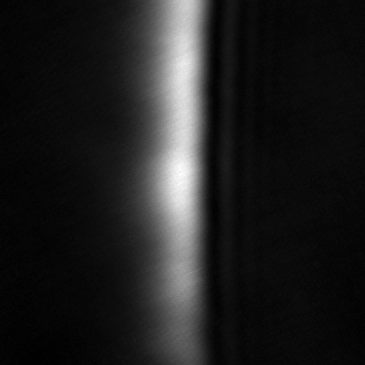
\includegraphics[width=4cm,keepaspectratio]{interference/figures/move/321-8.png}}
\subfigure[]{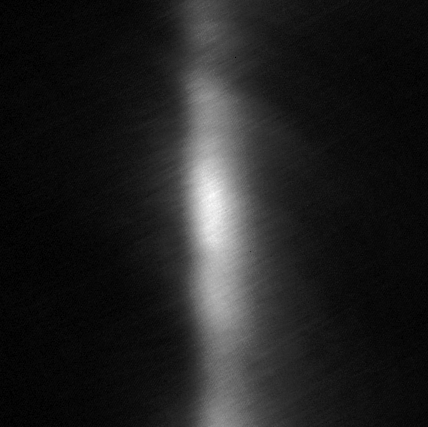
\includegraphics[width=4cm,keepaspectratio]{interference/figures/move/321-9.png}}\\
\caption{Images of the optical field for the section of the conically
scattered light as the focal plane of $f_4$ is moved from (a), best focus,
to (f), the far field.  All images have been normalized relative to
themselves.}
\label{fig:321up}
\end{figure}
